\documentclass[a4paper,titlepage]{article}

\usepackage{geometry}
\geometry{a4paper, left=10mm, right=10mm, top=10mm, bottom=15mm}

\usepackage[colorlinks=false]{hyperref}
\usepackage[utf8]{inputenc}
\usepackage{float}
\usepackage{pdfpages}
\usepackage{imakeidx}
%\usepackage{pdflscape}
\usepackage{graphicx}

\usepackage{listings}
\lstset{
	language=C++,
	basicstyle=\scriptsize\ttfamily,
    keywordstyle=\color{blue}\ttfamily,
    stringstyle=\color{red}\ttfamily,
    commentstyle=\color{red}\ttfamily,
    morecomment=[l][\color{red}]{\#},
    tabsize=2,
    frame=single,
    inputencoding=utf8,
    extendedchars=true,
    showstringspaces=false,
    breaklines=true
}

\lstset{literate=
  {á}{{\'a}}1 {é}{{\'e}}1 {í}{{\'i}}1 {ó}{{\'o}}1 {ú}{{\'u}}1
  {Á}{{\'A}}1 {É}{{\'E}}1 {Í}{{\'I}}1 {Ó}{{\'O}}1 {Ú}{{\'U}}1
  {à}{{\`a}}1 {è}{{\`e}}1 {ì}{{\`i}}1 {ò}{{\`o}}1 {ù}{{\`u}}1
  {À}{{\`A}}1 {È}{{\'E}}1 {Ì}{{\`I}}1 {Ò}{{\`O}}1 {Ù}{{\`U}}1
  {ä}{{\"a}}1 {ë}{{\"e}}1 {ï}{{\"i}}1 {ö}{{\"o}}1 {ü}{{\"u}}1
  {Ä}{{\"A}}1 {Ë}{{\"E}}1 {Ï}{{\"I}}1 {Ö}{{\"O}}1 {Ü}{{\"U}}1
  {â}{{\^a}}1 {ê}{{\^e}}1 {î}{{\^i}}1 {ô}{{\^o}}1 {û}{{\^u}}1
  {Â}{{\^A}}1 {Ê}{{\^E}}1 {Î}{{\^I}}1 {Ô}{{\^O}}1 {Û}{{\^U}}1
  {œ}{{\oe}}1 {Œ}{{\OE}}1 {æ}{{\ae}}1 {Æ}{{\AE}}1 {ß}{{\ss}}1
  {ç}{{\c c}}1 {Ç}{{\c C}}1 {ø}{{\o}}1 {å}{{\r a}}1 {Å}{{\r A}}1
  {€}{{\EUR}}1 {£}{{\pounds}}1
}

% remove the paragraph indentation
\setlength{\parindent}{0in}

\author{}
\title{AlgoLab AS 2014}
\date{\today}

\makeindex
\newcommand{\topic}[1]{\index{#1}#1}
%\newcommand{\expdf}[3]{\begin{landscape}\includepdf[nup=1x2, landscape=true, pages={-}, pagecommand={\subsection{#1}\textbf{Keywords:} #2}]{#3}\end{landscape}\newpage}
\newcommand{\expdf}[3]{\subsection{#1}\textbf{Keywords:} #2}

\begin{document}

\maketitle
\tableofcontents
\newpage
\setcounter{page}{1}

\newpage\section{ACM}
\expdf{Even Pairs}{\topic{Scanline}}{even-pairs/even_pairs.pdf}
\lstinputlisting{even-pairs/main.cpp}
\lstinputlisting{../eth-algolab-benji/even_pairs/even_pairs.cpp}

\expdf{Build The Sum}{}{build-the-sum/build_sum.pdf}
\lstinputlisting{build-the-sum/main.cpp}
\lstinputlisting{../eth-algolab-benji/build_the_sum/build_the_sum.cpp}

\expdf{Shelves}{}{shelves/shelves.pdf}
\lstinputlisting{shelves/main.cpp}
\lstinputlisting{../eth-algolab-benji/shelves/shelves.cpp}

\expdf{Checking Change}{\topic{Dynamic Programming}}{checking-change/checking_change.pdf}
\lstinputlisting{checking-change/main.cpp}
\lstinputlisting{../eth-algolab-benji/checking_change/checking_change.cpp}

\expdf{Even Matrices}{}{even-matrices/even_matrices.pdf}
% TODO \lstinputlisting{even-matrices/main.cpp}
\lstinputlisting{../eth-algolab-benji/even_matrices/even_matrices.cpp}

\expdf{Race Tracks}{\topic{BFS (Graph)}}{race-tracks/race_tracks.pdf}
\lstinputlisting{race-tracks/main.cpp}
\lstinputlisting{../eth-algolab-benji/race_tracks/race_tracks.cpp}

\expdf{Boats}{\topic{Custom compare}, \topic{Class with compare}, \topic{Uses class}, \topic{Greedy}}{boats/boats.pdf}
\lstinputlisting{boats/main.cpp}
\lstinputlisting{../eth-algolab-benji/boats/boats.cpp}

\expdf{Aliens}{\topic{Custom compare}, \topic{Compare function}, \topic{Compare struct}, \topic{Uses class}, \topic{Scanline}}{aliens/aliens.pdf}
\lstinputlisting{aliens/main.cpp}
\lstinputlisting{../eth-algolab-benji/aliens/aliens.cpp}

\expdf{Next Path}{\topic{Custom compare}, \topic{Compare struct}, \topic{BFS (Graph)}}{next-path/next_path.pdf}
\lstinputlisting{next-path/main.cpp}
\lstinputlisting{../eth-algolab-benji/next_path/next_path.cpp}

\newpage\section{Dynamic Programming}
\expdf{Longest Path}{\topic{BFS (Graph)}}{longest-path/longest_path.pdf}
\lstinputlisting{longest-path/main.cpp}
\lstinputlisting{../eth-algolab-benji/longest_path/longest_path.cpp}

\expdf{Light Pattern}{\topic{Scanline}}{light-pattern/light_pattern.pdf}
\lstinputlisting{light-pattern/main.cpp}
\lstinputlisting{../eth-algolab-benji/light_patterns/light_patern.cpp}

\expdf{Burning Coins}{\topic{Dynamic Programming}}{burning-coins/burning_coins.pdf}
\lstinputlisting{burning-coins/main.cpp}
\lstinputlisting{../eth-algolab-benji/burning_coins/burning_coins.cpp}

\expdf{Poker Chips}{\topic{Dynamic Programming}}{pokerchips/poker_chips.pdf}
\lstinputlisting{pokerchips/main.cpp}
\lstinputlisting{../eth-algolab-benji/poker_chips/poker_chips.cpp}

\newpage\section{BGL Introduction}
\expdf{Building a Graph}{\topic{Shortest path}, \topic{Spanning tree}, \topic{Graph with edge weight map}}{building-a-graph/bgl_intro.pdf}
% WRONG :) \lstinputlisting{building-a-graph/main.cpp}
\lstinputlisting{../eth-algolab-benji/building_a_graph/building_a_graph.cpp}

\expdf{Ant Challenge}{\topic{Spanning tree}, \topic{Shortest path}, \topic{Graph with edge index map}}{ant-challenge/ant_challenge.pdf}
\lstinputlisting{ant-challenge/main.cpp}
\lstinputlisting{../eth-algolab-benji/ant_challenge/ant_challenge.cpp}

\expdf{Important Bridges}{\topic{Articulation points}, \topic{Biconnected components}}{important-bridges/important_bridges.pdf}
\lstinputlisting{important-bridges/main.cpp}
\lstinputlisting{../eth-algolab-benji/important_bridges/important_bridges.cpp}

\expdf{Shy Programmers}{\topic{Planarity}}{shy-programmers/shy_programmers.pdf}
\lstinputlisting{shy-programmers/main.cpp}
\lstinputlisting{../eth-algolab-benji/shy_programmers/shy_programmers.cpp}

\expdf{Fluid Borders}{\topic{Planarity}}{fluid-borders/fluid-borders.pdf}
\lstinputlisting{fluid-borders/main.cpp}
\lstinputlisting{../eth-algolab-benji/fluid_borders/fluid_borders.cpp}

\newpage\section{Flows and Matchings}
\expdf{Buddies Selection}{\topic{Matching}, \topic{Match size}}{buddy-selection/buddies.pdf}
\lstinputlisting{buddy-selection/main.cpp}
\lstinputlisting{../eth-algolab-benji/buddies/buddies.cpp}

\expdf{Satellites}{\topic{Matching}, \topic{DFS (Graph)}, \topic{Matching with DFS}}{satellites/satellites.pdf}
\lstinputlisting{satellites/main.cpp}
\lstinputlisting{../eth-algolab-benji/satellites/satellites.cpp}

\expdf{Coin Tossing}{\topic{Graph with edge capacity}, \topic{Graph with residual capacity}, \topic{Graph with reverse edges}, \topic{Custom add edge function}, \topic{Max-flow}}{coin-tossing/cointossing.pdf}
\lstinputlisting{coin-tossing/main.cpp}
\lstinputlisting{../eth-algolab-benji/coin_tossing/coin_tossing.cpp}

\expdf{Kingdom Defence}{\topic{Graph with edge capacity}, \topic{Graph with residual capacity}, \topic{Graph with reverse edges}, \topic{Max-flow}, \topic{Custom add edge function} inlined by hand}{kingdom-defence/defence.pdf}
\lstinputlisting{kingdom-defence/main.cpp}
\lstinputlisting{../eth-algolab-benji/kingdom_defense/kingdom_defense.cpp}

\expdf{The Great Game}{\topic{Dynamic Programming}}{the-great-game/great_game.pdf}
\lstinputlisting{the-great-game/main.cpp}
\lstinputlisting{../eth-algolab-benji/the_great_game/the_great_game.cpp}

\expdf{Surveillance Photographs}{\topic{Graph with edge capacity}, \topic{Graph with residual capacity}, \topic{Graph with reverse edges}, \topic{Custom add edge function}, \topic{Max-flow}}{surveillance-photographs/surveillance.pdf}
\lstinputlisting{surveillance-photographs/main.cpp}
\lstinputlisting{../eth-algolab-benji/surveillance_photographs/surveillance.cpp}

\newpage\section{CGAL Introduction}
\expdf{Hit?}{\topic{CGAL Segment}, \topic{CGAL Ray}, \topic{CGAL do\_intersect}}{hit/hit.pdf}
\lstinputlisting{hit/main.cpp}
\lstinputlisting{../eth-algolab-benji/hit/hit.cpp}

\expdf{Antenna}{\topic{floor\_to\_double}, \topic{ceil\_to\_double}, \topic{Minimal Circle}, \topic{CGAL sqrt}}{antenna/antenna.pdf}
\lstinputlisting{antenna/main.cpp}
\lstinputlisting{../eth-algolab-benji/antenna/antenna.cpp}

\expdf{First Hit}{\topic{CGAL randomise}, \topic{CGAL intersection}}{first-hit/first_hit.pdf}
\lstinputlisting{first-hit/main.cpp}
\lstinputlisting{../eth-algolab-benji/first_hit/first_hit.cpp}

\expdf{Almost Antenna}{\topic{CGAL qrt}, \topic{Minimal Circle}, \topic{floor\_to\_double}, \topic{ceil\_to\_double}}{almost-antenna/almost_antenna.pdf}
\lstinputlisting{almost-antenna/main.cpp}
\lstinputlisting{../eth-algolab-benji/almost_antenna/almost_antenna.cpp}

\newpage\section{Proximity Structures}
\expdf{Graypes}{\topic{setprecision}, \topic{Delaunay Triangulation}, \topic{Finite edge iteration}}{graypes/graypes.pdf}
\lstinputlisting{graypes/main.cpp}
\lstinputlisting{../eth-algolab-benji/graypes/graypes.cpp}

\expdf{Bistro}{\topic{Delaunay Triangulation}}{bistro/bistro.pdf}
\lstinputlisting{bistro/main.cpp}
\lstinputlisting{../eth-algolab-benji/bistro/bistro.cpp}

\expdf{H1N1}{\topic{Delaunay Triangulation}, \topic{CGAL Triangulation with DFS}, \topic{Finite face iteration}}{h1n1/H1N1.pdf}
\lstinputlisting{h1n1/main.cpp}
\lstinputlisting{../eth-algolab-benji/h1n1/h1n1.cpp}

\expdf{Germs}{\topic{Delaunay Triangulation}, \topic{Finite vertices iteration}, \topic{Finite edge iteration}, \topic{Iteration over std::map}}{germs/germs.pdf}
\lstinputlisting{germs/main.cpp}
\lstinputlisting{../eth-algolab-benji/germs/germs.cpp}

\expdf{Hiking Maps}{\topic{Delaunay Triangulation}, \topic{CGAL turn function}, \topic{CGAL right\_turn}, \topic{Scanline}}{hiking-maps/potw7.pdf}
% TODO \lstinputlisting{hiking-maps/main.cpp}
\lstinputlisting{../eth-algolab-benji/hiking_maps/hiking.cpp}

\newpage\section{Linear/Quadratic Programming}
\expdf{What is the Maximum?}{\topic{Quadratic Program}, \topic{ceil\_to\_double}, \topic{floor\_to\_double}}{maximize-it/maximizeit.pdf}
\lstinputlisting{maximize-it/main.cpp}
% TODO: \lstinputlisting{../eth-algolab-benji/}

\expdf{Diets}{\topic{Quadratic Program}, \topic{Non-negative quadratic program}}{diets/diet.pdf}
\lstinputlisting{diets/main.cpp}
\lstinputlisting{../eth-algolab-benji/diet/diet.cpp}

\expdf{Portfolios}{\topic{Quadratic Program}}{portfolio/portfolios.pdf}
\lstinputlisting{portfolio/main.cpp}
\lstinputlisting{../eth-algolab-benji/portfolios/portfolios.cpp}

\expdf{Inball}{\topic{Quadratic Program}, \topic{Quadratic Program: Maximize}}{inball/inball.pdf}
\lstinputlisting{inball/main.cpp}
\lstinputlisting{../eth-algolab-benji/inball/inball.cpp}

\expdf{Collisions}{\topic{Point set}, \topic{Delaunay Triangulation}, \topic{Finite edge iteration}, \topic{Triangulation with info()}}{collisions/collisions.pdf}
\lstinputlisting{collisions/main.cpp}
\lstinputlisting{../eth-algolab-benji/collisions/collisions.cpp}

\newpage\section{Exam Preparation}
\expdf{TheeV}{\topic{CGAL}, \topic{Minimal Circle}, \topic{Custom compare}, \topic{Compare function}, \topic{Binary search}}{theev/TheeV.pdf}
\lstinputlisting{theev/main.cpp}
\lstinputlisting{../eth-algolab-benji/thee_v/thee.cpp}

\expdf{Algocoön Group}{\topic{BGL}, \topic{Graph with edge capacity}, \topic{Graph with residual capacity}, \topic{Graph with reverse edges}, \topic{Max-flow}}{algocoon-group/algocoon.pdf}
\lstinputlisting{algocoon-group/main.cpp}
\lstinputlisting{../eth-algolab-benji/algocoon/algocoon.cpp}

\expdf{Monkey Island}{\topic{BGL}, \topic{Strong component}, \topic{Edge iteration}, \topic{Uses class}, \topic{Custom compare}, \topic{Compare function}, \topic{Greedy}, \topic{DFS (Graph)}}{monkey-island/monkey_island.pdf}
\lstinputlisting{monkey-island/main.cpp}
\lstinputlisting{../eth-algolab-benji/monkey_island/monkey_island.cpp}

\expdf{Odd Route}{\topic{ACM}, \topic{BFS (Graph)}, \topic{Custom BFS}}{odd-route/odd_route.pdf}
\lstinputlisting{odd-route/main.cpp}
\lstinputlisting{../eth-algolab-benji/odd_route/odd_route.cpp}

\expdf{Divisor Distance}{\topic{Prime Sieve}, \topic{Next Prime}, \topic{ACM}}{divisor-distance/divisor_distance.pdf}
\lstinputlisting{divisor-distance/main.cpp}
\lstinputlisting{../eth-algolab-benji/divisor_distance/divisor_distance.cpp}

\expdf{Portfolios Revisited}{\topic{CGAL}, \topic{Quadratic Program}, \topic{Non-negative quadratic program}, \topic{Exponential bound search}, \topic{Binary search}}{portfolios-revisited/portfolios-revisited.pdf}
\lstinputlisting{portfolios-revisited/main.cpp}
\lstinputlisting{../eth-algolab-benji/portfolios_revisited/portfolios_rev.cpp}

\expdf{Tetris}{\topic{BGL}, \topic{Graph with edge capacity}, \topic{Graph with residual capacity}, \topic{Graph with reverse edges}, \topic{Max-flow}}{tetris/tetris.pdf}
\lstinputlisting{tetris/main.cpp}
\lstinputlisting{../eth-algolab-benji/tetris/tetris.cpp}

\expdf{Stamp Exhibition}{\topic{CGAL}, \topic{Quadratic Program}}{stamp-exhibition/stamps.pdf}
\lstinputlisting{stamp-exhibition/main.cpp}
\lstinputlisting{../eth-algolab-benji/stamp_exhibition/stamps.cpp}

\expdf{Placing Knights}{\topic{BGL}, \topic{Matching}}{placing-knights/placing-knights.pdf}
\lstinputlisting{placing-knights/main.cpp}
\lstinputlisting{../eth-algolab-benji/placing_knights/placing_knights.cpp}

\expdf{Beach Bar}{\topic{ACM}, \topic{Scanline}}{beach-bars/beach_bar.pdf}
\lstinputlisting{beach-bars/main.cpp}
\lstinputlisting{../eth-algolab-benji/beach_bar/beach_bar.cpp}

\expdf{Light the Stage}{\topic{CGAL}, \topic{Point set}, \topic{Triangulation with info()}}{light-the-stage/ex3.pdf}
\lstinputlisting{light-the-stage/main.cpp}
\lstinputlisting{../eth-algolab-benji/light_the_stage/light_the_stage.cpp}

\expdf{Search Snippets}{\topic{ACM}, \topic{Scanline}, \topic{Custom compare}, \topic{Compare in class}}{search-snippets/snippets.pdf}
\lstinputlisting{search-snippets/main.cpp}
\lstinputlisting{../eth-algolab-benji/search_snippets/search_snippet.cpp}

\expdf{Radiation Therapy}{\topic{CGAL}, \topic{Quadratic Program}, \topic{Exponential bound search}, \topic{Binary search}}{radiation-therapy/radiation1.pdf}
\lstinputlisting{radiation-therapy/main.cpp}
\lstinputlisting{../eth-algolab-benji/radiation_therapy/radiation.cpp}

\expdf{Island Hopping}{\topic{ACM}, \topic{Dynamic Programming}}{island-hopping/islandhopping.pdf}
\lstinputlisting{island-hopping/main.cpp}
\lstinputlisting{../eth-algolab-benji/island_hopping/island_hopping.cpp}

\expdf{Sweepers}{\topic{BGL}, \topic{Graph with edge capacity}, \topic{Graph with residual capacity}, \topic{Graph with reverse edges}, \topic{Max-flow}, \topic{Euler circuit}, \topic{Components}}{sweepers/sweepers.pdf}
\lstinputlisting{sweepers/main.cpp}
\lstinputlisting{../eth-algolab-benji/sweepers/sweepers.cpp}

\expdf{Clues}{\topic{BGL}, \topic{CGAL}, \topic{BGL with CGAL}, \topic{CGAL with BGL}, \topic{Point set}, \topic{Triangulation with info()}, \topic{Bipartite}, \topic{Components}}{clues/potw12.pdf}
\lstinputlisting{clues/main.cpp}
\lstinputlisting{../eth-algolab-benji/clues/clues.cpp}

\expdf{Radiation 2}{\topic{CGAL}, \topic{Delaunay Triangulation}, \topic{Point set}, \topic{Triangulation with info()}}{radiation2/radiation2.pdf}
\lstinputlisting{radiation2/main.cpp}
% TODO: \lstinputlisting{../eth-algolab-benji/radiation_2/}

\expdf{Knights}{\topic{BGL}, \topic{Graph with edge capacity}, \topic{Graph with residual capacity}, \topic{Graph with reverse edges}, \topic{Max-flow}}{knights/knights.pdf}
\lstinputlisting{knights/main.cpp}
\lstinputlisting{../eth-algolab-benji/knights/knights.cpp}

\expdf{Tight Words}{\topic{ACM}, \topic{Dynamic Programming}}{tight-words/tight_words.pdf}
\lstinputlisting{tight-words/main.cpp}
\lstinputlisting{../eth-algolab-benji/tight_words/tight_words.cpp}

\expdf{Cantonal Courier}{\topic{BGL}, \topic{Graph with edge capacity}, \topic{Graph with residual capacity}, \topic{Graph with reverse edges}, \topic{Max-flow}}{cantonal-courier/courier.pdf}
\lstinputlisting{cantonal-courier/main.cpp}
\lstinputlisting{../eth-algolab-benji/cantonal_courier/courier.cpp}

\section{Useful Snippets and Stuff}
\subsection{General remarks}
\begin{itemize}
\item around $10'000'000$ operations/iterations per second (ACM slide below claims its less, but oh well)
\end{itemize}
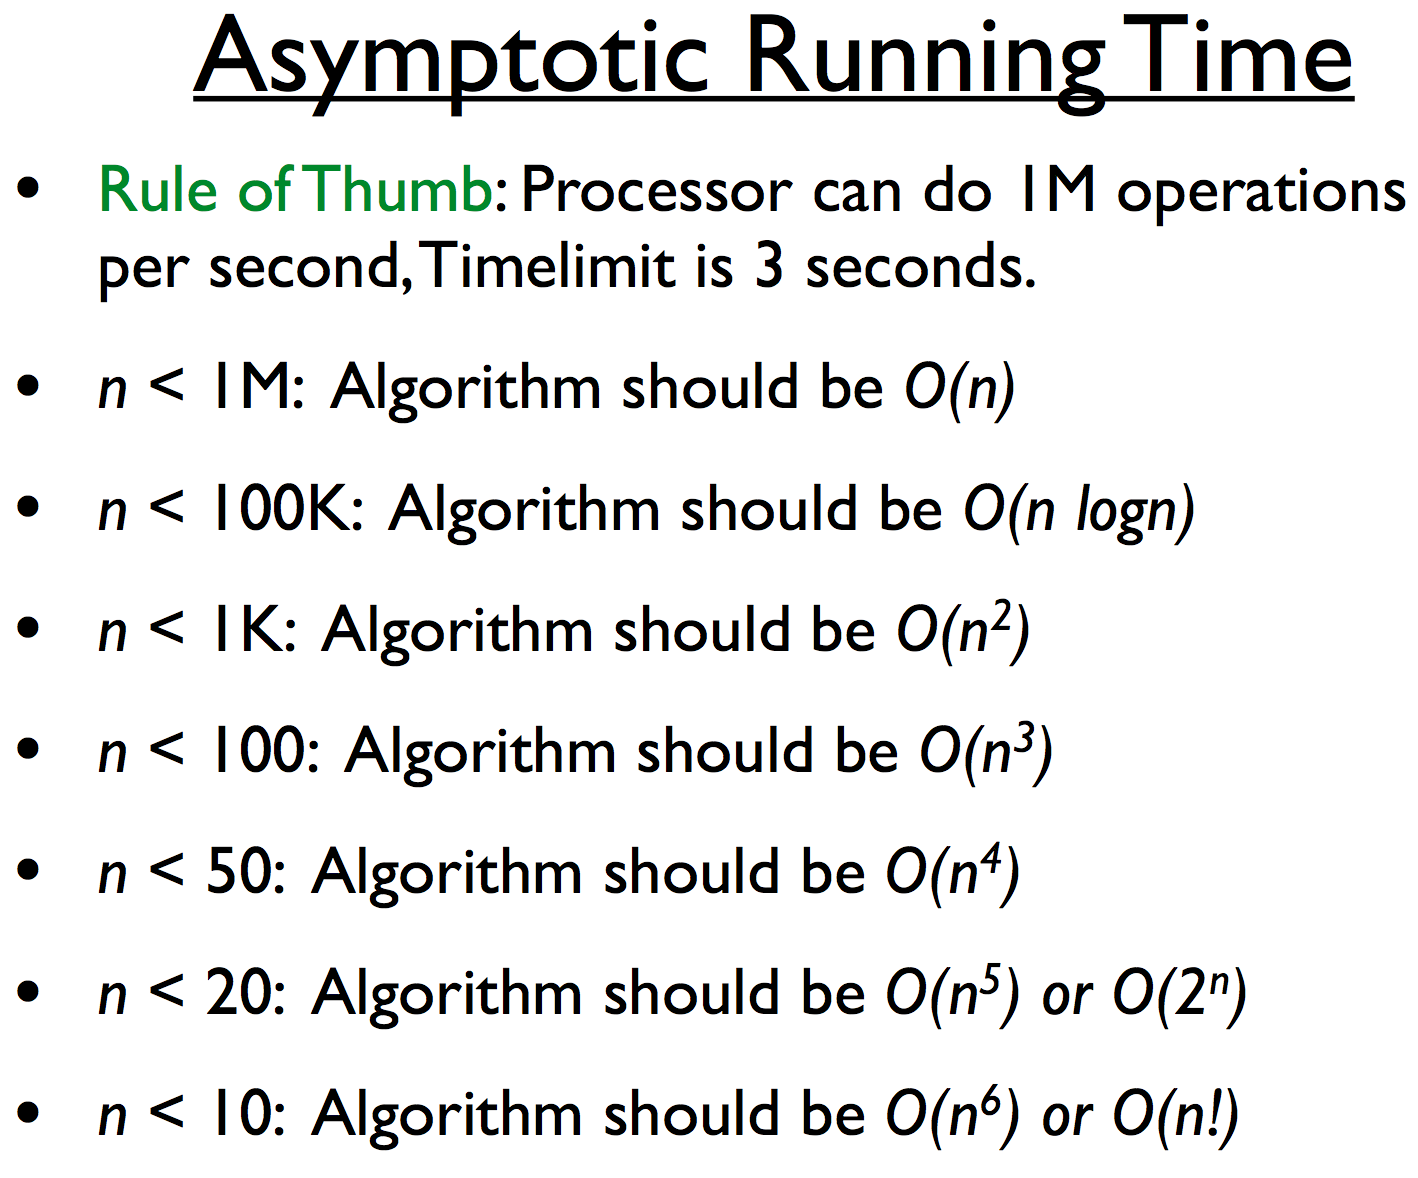
\includegraphics[scale=0.2]{_useful-snippets/general0.png}

\subsection{Custom Sorting}
\lstinputlisting{_useful-snippets/sort.cpp}

\subsection{CMake Configuration}
Add to \texttt{CMakeLists.txt}:
\lstinputlisting{_useful-snippets/cmakelists.txt}

Debugging can also be enabled by calling \texttt{cmake -DCMAKE\_BUILD\_TYPE=Debug}, however this adds only the \texttt{-g} flag!

\subsection{CMake and CGAL}
\begin{lstlisting}
# Step 0: IMPORTANT: first, create the C++ source code file

# Step 1: call CGAL CMake script
cgal_create_cmake_script

# Step 2: modify CMakeLists.txt if needed (adding C++11 support, debugging, etc.)
vim CMakeLists.txt
# or
nano CMakeLists.txt
# or ...

# Step 3: call CMake, don't forget the dot
cmake .

# Step 4: from now on always enough to call make
make

# Step 5: execute application
\end{lstlisting}

\subsection{BGL}
URL for normal graph functions: \url{https://judge.inf.ethz.ch/doc/boost/libs/graph/doc/graph_concepts.html}. Also good starting point is the ``A Quick Tour of the Boost Graph Library'' (see TOC).

\lstinputlisting{_useful-snippets/bgl.cpp}

\subsection{CGAL: Linear/Quadratic Programming}
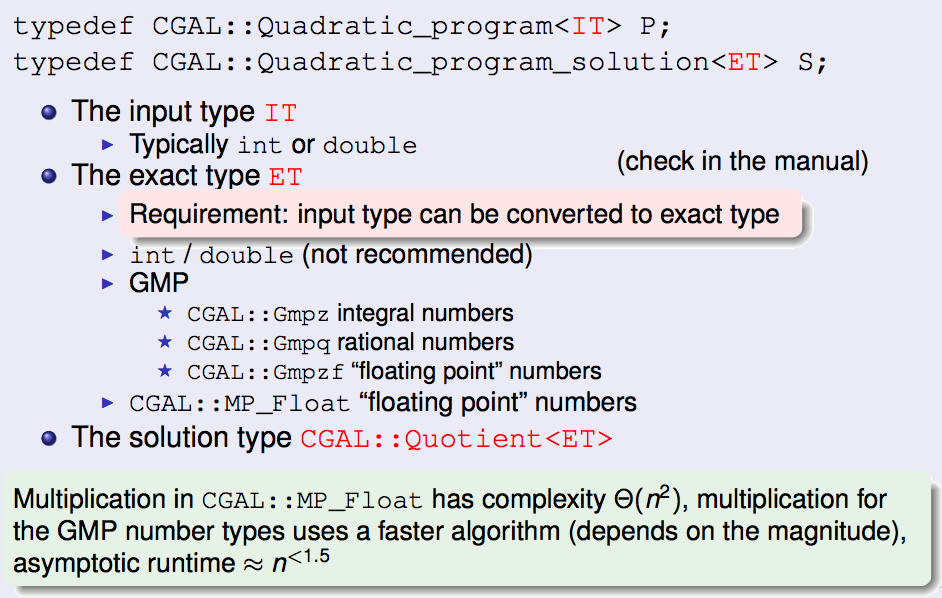
\includegraphics{_useful-snippets/lp_qp0.png}\\
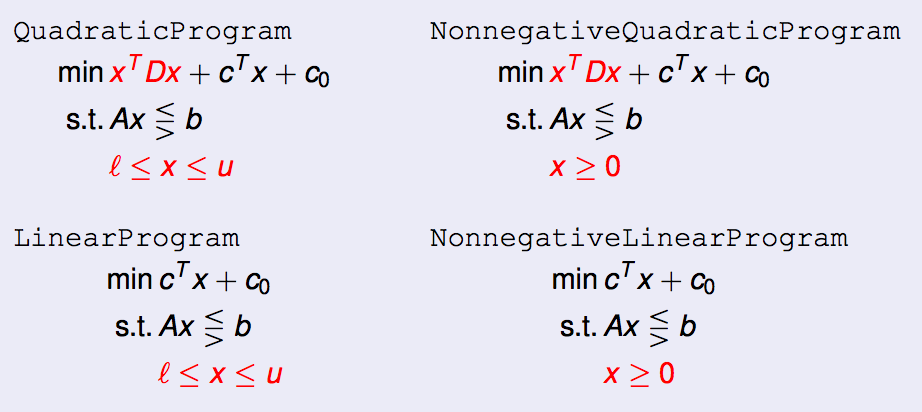
\includegraphics{_useful-snippets/lp_qp1.png}\\
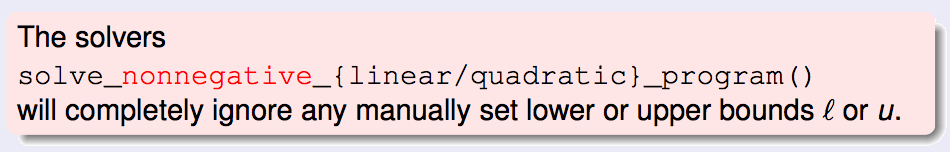
\includegraphics{_useful-snippets/lp_qp2.png}\\
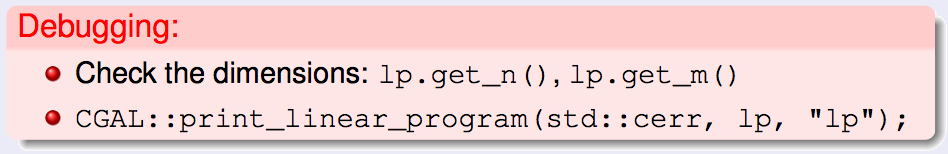
\includegraphics{_useful-snippets/lp_qp3.png}\\
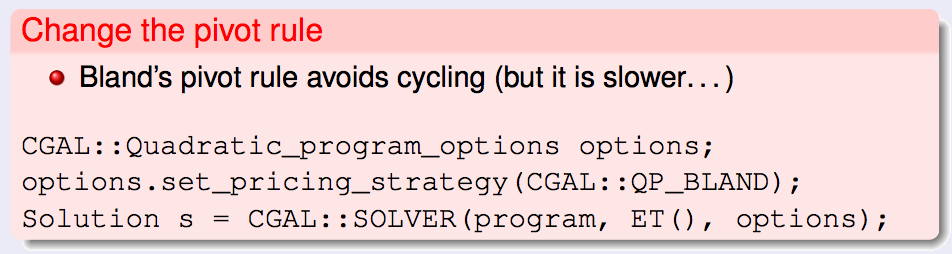
\includegraphics{_useful-snippets/lp_qp4.png}\\
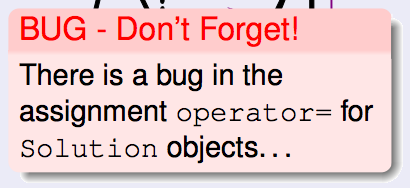
\includegraphics{_useful-snippets/lp_qp5.png}

\subsection{CGAL: Approximation (Triangulation)}
Nex image `\texttt{f}' is a `\texttt{face handle}'\\
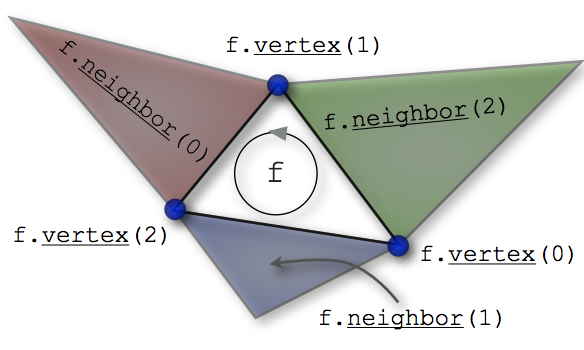
\includegraphics{_useful-snippets/cgal0.png}\\
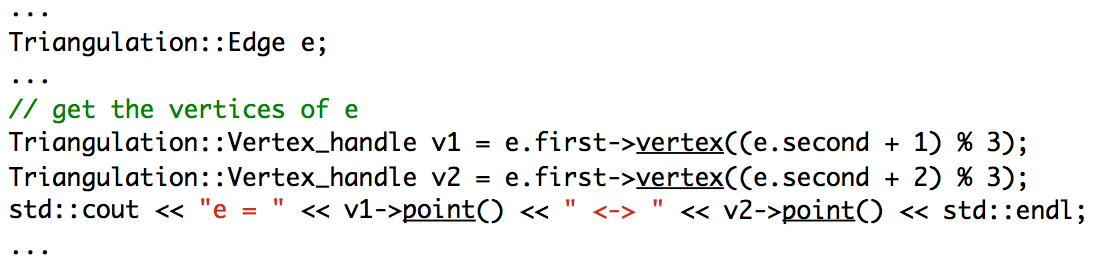
\includegraphics{_useful-snippets/cgal1.png}

\subsection{Matching}
\begin{itemize}
\item Undirected graph $G = (V, E)$
\item Is a subset $M \subseteq E$ of edges
\item Each pair of edges of the matching set ($e_1, e_2 \in M$) don't have a common vertices $v \in V$
\item Or based on the vertices: Every pair of vertices $v_1, v_2 \in V$ aren't the start or end point of an edge $e \in M$
\item \textbf{Maximal Matching}: If it's not possible to add another edge $e \in E \\ M$ to $M$ and $M$ being a matching
\item \textbf{Maximum Matching}/\textbf{Maximum Cardinality Matching}: A maximal matching with the largest amount of edges. There might exists multiple maximum matchings.
\end{itemize}

\subsection{Vertex Cover}
\begin{itemize}
\item Undirected graph $G = (V, E)$
\item A vertex cover is a subset $V' \subseteq V$ such that for each edge $(u, v) =: e \in E$ $u \in V'$ and/or $v \in V'$
\item \textbf{Minimal Vertex Cover}: Generally NP-complete. Is the smallest possible vertex cover.
\end{itemize}

\subsection{König's Theorem}
\begin{itemize}
\item only for bipartite graphs
\item The size of a maximum matching (maximum cardinality matching) is equal to the minimal vertex cover
\end{itemize}

Algorithm:
\begin{enumerate}
\item Let $G = (V, E)$ be a undirected bipartite graph, i.e. $L \cup R = V \land L \cap R = \emptyset$
\item Calculate the Maximum Matching (Maximum Cardinality Matching), resulting in a matching $M \subseteq E$
\item Mark all vertices $v \in L$ that are not in $M$ ($v \notin M$) as visited
\item Start at visited vertices and do a vertices search (DFS) from $L$ to $R$ along edges from $V \ M$ and $R$ to $L$ along edges from $M$. Each such visited vertex is marked as visited
\item All unvisited vertices in $L$ and all visited in $R$ are part of the minimal vertex cover
\end{enumerate}

\subsection{Connected Component}
\begin{itemize}
\item For undirected graphs
\item Connected component is a subgraph of a graph where any two vertices in the subgraph are connected by a path, but no path exists to vertices to ones outside the subgraph
\end{itemize}

\subsection{Strongly Connected Component}
\begin{itemize}
\item For directed graphs
\item Partitions a graph into subgraphs where each subgraph is strongly connected.
\item \textbf{Strongly Connected}: A graph is strongly connected iff every vertex of the graph is reachable from every other vertex
\end{itemize}

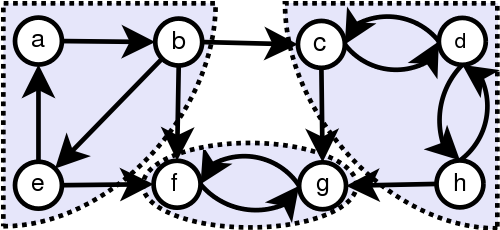
\includegraphics[scale=0.4]{_useful-snippets/graph0.png}\\
From: \url{https://commons.wikimedia.org/wiki/File:Scc.png}

\subsection{Biconnected Component / Articulation Points}
See BGL documentation, it's pretty good. Otherwise this might help:
\begin{itemize}
\item \textbf{Biconnected Graph}: A connected graph is biconnected iff removing any single vertex (and all edges from/to this vertex) can't disconnect the graph. Such a graph doesn't contain \textit{articulation points}!
\item \textbf{Biconnected Components}: A subset of vertices where removing one of these vertices doesn't result in a disconnected graph inside the subgraph. Vertices can belong to multiple biconnected components!
\item \textbf{Articulation Points}: These are the vertices that belong to more than one biconnected component. Such vertices are called \textit{articulation points}. Removing such a articulation point would result in an increase of connected components (i.e. increase the number of graphs). No such articulation points means the graph is biconnected!
\end{itemize}

\subsection{BGL: DFS / BFS}
\lstinputlisting{_useful-snippets/bgl_dfs_bfs.cpp}
\begin{lstlisting}
# OUTPUT
Depth First Search:
here do some initialisation before passing to depth_first_search()
initialize_vertex() for vertex: 0
initialize_vertex() for vertex: 1
initialize_vertex() for vertex: 2
initialize_vertex() for vertex: 3
initialize_vertex() for vertex: 4
initialize_vertex() for vertex: 5
initialize_vertex() for vertex: 6
initialize_vertex() for vertex: 7
start_vertex() for vertex: 0
discover_vertex() for vertex: 0
examine_edge() for edge: (0,1)
tree_edge() for edge: (0,1)
discover_vertex() for vertex: 1
examine_edge() for edge: (1,0)
back_edge() for edge: (1,0)
examine_edge() for edge: (1,3)
tree_edge() for edge: (1,3)
discover_vertex() for vertex: 3
examine_edge() for edge: (3,1)
back_edge() for edge: (3,1)
finish_vertex() for vertex: 3
examine_edge() for edge: (1,4)
tree_edge() for edge: (1,4)
discover_vertex() for vertex: 4
examine_edge() for edge: (4,1)
back_edge() for edge: (4,1)
examine_edge() for edge: (4,6)
tree_edge() for edge: (4,6)
discover_vertex() for vertex: 6
examine_edge() for edge: (6,4)
back_edge() for edge: (6,4)
finish_vertex() for vertex: 6
finish_vertex() for vertex: 4
finish_vertex() for vertex: 1
finish_vertex() for vertex: 0
start_vertex() for vertex: 2
discover_vertex() for vertex: 2
examine_edge() for edge: (2,5)
tree_edge() for edge: (2,5)
discover_vertex() for vertex: 5
examine_edge() for edge: (5,2)
back_edge() for edge: (5,2)
finish_vertex() for vertex: 5
finish_vertex() for vertex: 2
start_vertex() for vertex: 7
discover_vertex() for vertex: 7
finish_vertex() for vertex: 7


Breath First Search
here do some initialisation before passing to breadth_first_search()
initialize_vertex() for vertex: 0
initialize_vertex() for vertex: 1
initialize_vertex() for vertex: 2
initialize_vertex() for vertex: 3
initialize_vertex() for vertex: 4
initialize_vertex() for vertex: 5
initialize_vertex() for vertex: 6
initialize_vertex() for vertex: 7
discover_vertex() for vertex: 0
examine_vertex() for vertex: 0
examine_edge() for edge: (0,1)
tree_edge() for edge: (0,1)
discover_vertex() for vertex: 1
finish_vertex() for vertex: 0
examine_vertex() for vertex: 1
examine_edge() for edge: (1,0)
non_tree_edge() for edge: (1,0)
black_target() for edge: (1,0)
examine_edge() for edge: (1,3)
tree_edge() for edge: (1,3)
discover_vertex() for vertex: 3
examine_edge() for edge: (1,4)
tree_edge() for edge: (1,4)
discover_vertex() for vertex: 4
finish_vertex() for vertex: 1
examine_vertex() for vertex: 3
examine_edge() for edge: (3,1)
non_tree_edge() for edge: (3,1)
black_target() for edge: (3,1)
finish_vertex() for vertex: 3
examine_vertex() for vertex: 4
examine_edge() for edge: (4,1)
non_tree_edge() for edge: (4,1)
black_target() for edge: (4,1)
examine_edge() for edge: (4,6)
tree_edge() for edge: (4,6)
discover_vertex() for vertex: 6
finish_vertex() for vertex: 4
examine_vertex() for vertex: 6
examine_edge() for edge: (6,4)
non_tree_edge() for edge: (6,4)
black_target() for edge: (6,4)
finish_vertex() for vertex: 6
\end{lstlisting}

\subsection{Sorting Algorithms Implemented}
\lstinputlisting{_useful-snippets/sort_algos.cpp}

\newpage
\printindex


\end{document}